%\ctparttext{\color{black}\begin{center}
%		Esta es una descripción de la parte de informática.
%\end{center}}

%\part{Parte de informática}
\chapter{Análisis y diseño}


\section{Objetivos y análisis de requisitos}

Los objetivos que se persiguen al realizar este proyecto son realizar un estudio de distintos modelos de epidemiología, comprendiendo cómo afectan sus parámetros y condiciones iniciales a la evolución en el tiempo de estos modelos, desde un punto de vista tanto teórico como práctico, apoyándonos en distintas gráficas interactivas para ilustrar dichos comportamientos. Asimismo, se va a analizar la bondad de ajustes de parámetros de algunos de los modelos presentados aplicados a datos reales, comprobando cuáles proporcionan mejores resultados en cada caso. Con el fin de satisfacer todos estos objetivos, se ha extraído la siguiente lista de requisitos:

\begin{itemize}
\item \textbf{Requisitos funcionales}
	\begin{itemize}
	\item Se debe poder modificar los parámetros de las gráficas de los distintos modelos.
	\item El usuario debe poder elegir con qué modelo quiere trabajar.
	\item El sistema debe permitir descargar las imágenes de las gráficas obtenidas.
	\item El sistema debe poder cargar y leer ficheros de datos.
	\item Se debe visualizar el ajuste obtenido mediante gráficas.
	\end{itemize}
\item \textbf{Requisitos no funcionales}
	\begin{itemize}
	\item No se podrán ajustar datos de más de un fichero a la vez.
	\item Las gráficas deben ser en tiempo real
	\item Se mostrará información de ayuda, en caso de ser necesaria.
	\item Se debe poder usar desde el navegador.
	\end{itemize}
\item \textbf{Requisitos de información}
	\begin{itemize}
	\item Los ficheros de datos con los que se va a trabajar deben ser formato csv con una estructura específica.
	\end{itemize}
	\item Los valores decimales de los parámetros deben poder introducirse usando ',' o '.' como separadores.
\end{itemize}

\section{Desarrollo del proyecto}

Actualmente hay diversas metodologías de desarrollo del software. Cada uno de estos modelos consta de una serie de etapas en las que se ha dividido el desarrollo.

Para este proyecto, se ha optado por el modelo en espiral. En este modelo el software se desarrolla de forma incremental, es decir, se van añadiendo funcionalidades y mejoras al software según se van evaluando las que ya tiene. Cada bucle o iteración representa un conjunto de actividades. Estas actividades no están fijadas a ninguna prioridad, sino que las siguientes se eligen en función del análisis de riesgo, comenzando por el bucle interior. \eqref{modelo_espiral}

\begin{figure}
\begin{center}
\caption{Modelo en espiral.}
\label{modelo_espiral}
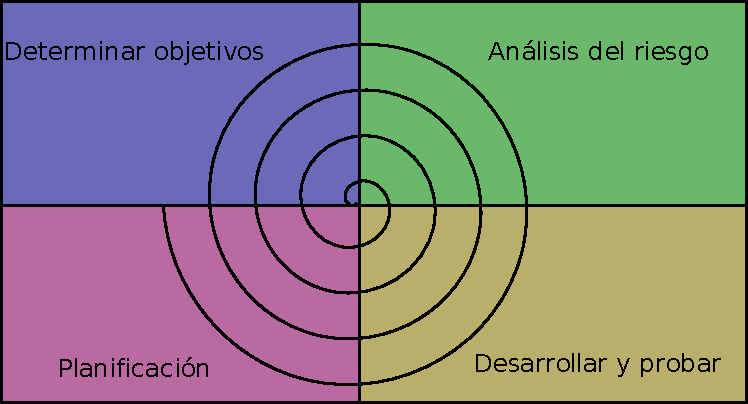
\includegraphics[scale=1]{modelo_espiral}
\end{center}
\end{figure}







